\section{The SCR Simulator} \label{sec:sim}

We have a simulator made in Unity by one of our members for the explicit purpose of this team, so it satisfies everything we could want from a simulator. It integrates with ROS, so it publishes simulated sensor data via ROS topics the same way the actual sensors do. This means we can run our code with no modifications whatsoever. The control node publishes motor commands, and these commands are received by the simulator in the same way they would be on the physical robot.

This simulator also has capabilities for environment and robot customization, so we're able to update it and increase the accuracy of our testing as we finalize the size and shape of the robot, and we're able to test different light levels, lane configurations, obstacle densities, and whatever else we want.

\begin{figure}[h]
    \centering
    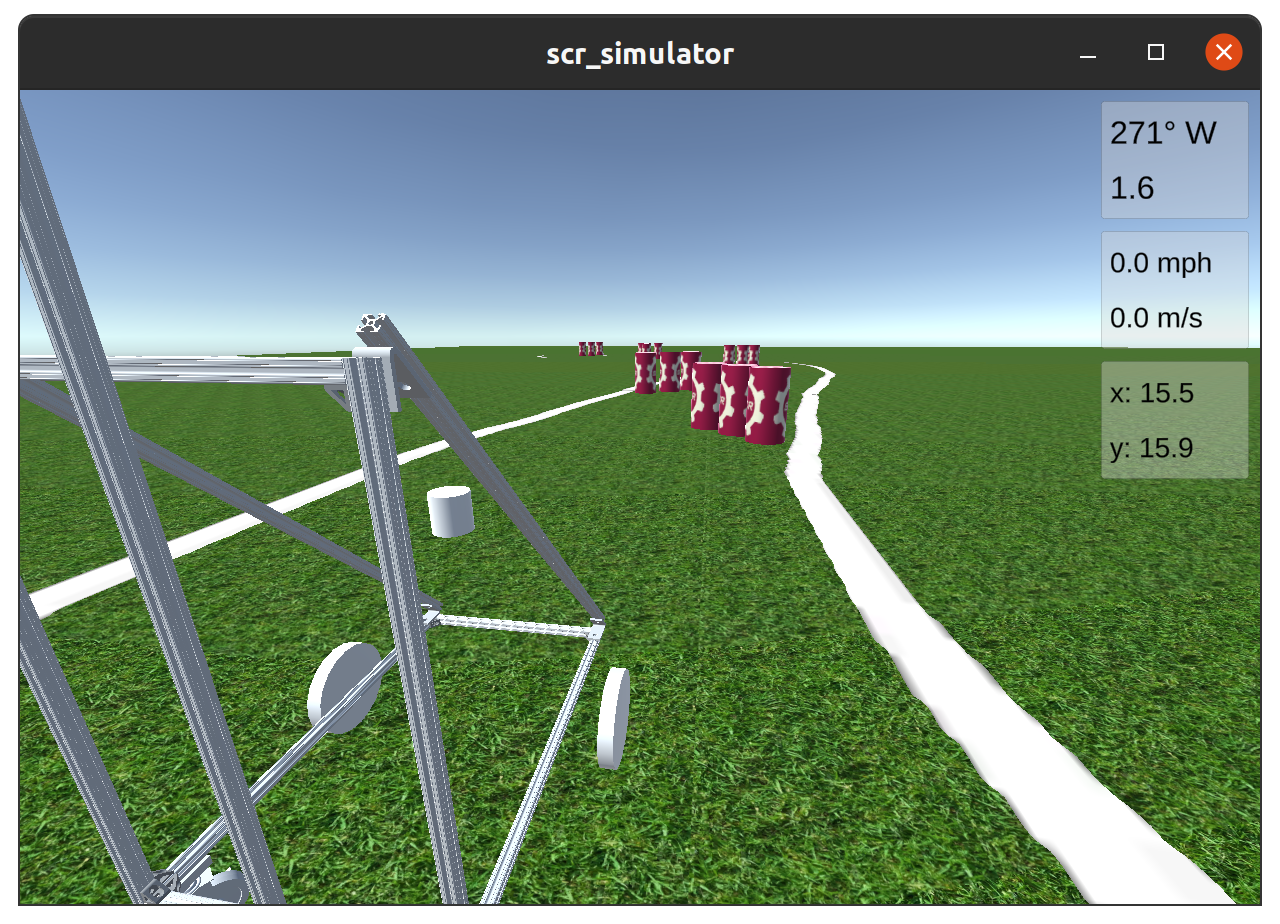
\includegraphics[width=0.6\textwidth]{images/software/sim_screenshot.png}
    \caption{Screenshot of the simulator on a map that contains both lanes and barrels.}
\end{figure}

The simulator has allowed us to make significant software progress without waiting for the robot to be built and wired, which allowed us to accomplish far more in parallel than we would have without it. We could develop our architecture and test different lane detection methods, which allowed us to settle on using a CNN and have plenty of time to flesh it out before we were setup to gather real camera footage for training data.

The simulator source code can be viewed and the latest release can be downloaded at \url{https://github.com/SoonerRobotics/scr_simulator}.